
\indent \indent
After the optimization of the variables during cross validation phase of the experiment the network is retrained using all the available signal.  The remaining portion of the signal excluding the data for last 31 days is used to make the extended system states. These extended systems states and the computed $\textbf{W}^{out}$ is used to make prediction using Equation \ref{eq:prediction}. \\
There are 31 output neurons each of which makes the prediction for $n=1\hdots,31$ days ahead. The network optimized during cross validation phase and retrained afterwards us used to make the prediction for the number of views for the month of December 2016. The accuracy of each of prediction range is calculated as NRMSE. These error measures are plotted in the Figure \ref{fig:nrmsevspw}. The predicted number of views and the actual number of views for different prediction horizon are plotted in figure \ref{fig:realvspredicted}
\\
The optimizable parameters that worked best for this experiment are presented in the table \ref{table:optimized}.

	\begin{center}
	\captionof{table}{Optimized values for control parameters} \label{table:optimized} 
	\begin{tabular}{|c|c|c|} \hline
		Parameters & Wikipedia Page No.12 & Wikipedia Page No.15\\ \hline
		$sf^{\mathbf{W}}$& 1.0& 2.2\\ \hline
		$sf^{\mathbf{Win}}$& 1.9 &2.1\\ \hline
		$sf^{\mathbf{B}}$& 1.4&1.5\\ \hline
		$\alpha$& 5.05 &0.0001\\ \hline
	\end{tabular}
	\end{center}
	

  \begin{figure}[h]
     \centering
     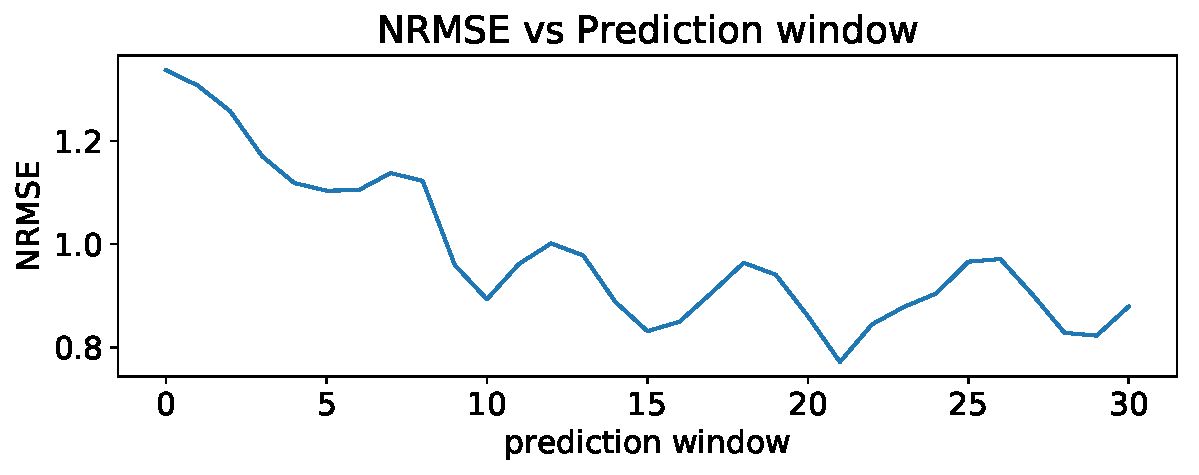
\includegraphics[width=\textwidth]{./results/images/nrmsevspwrec}

      \caption{NRMSE for different prediction window ranges}\label{fig:nrmsevspw}
  \end{figure}
 
 \begin{figure}[h]
    \centering
    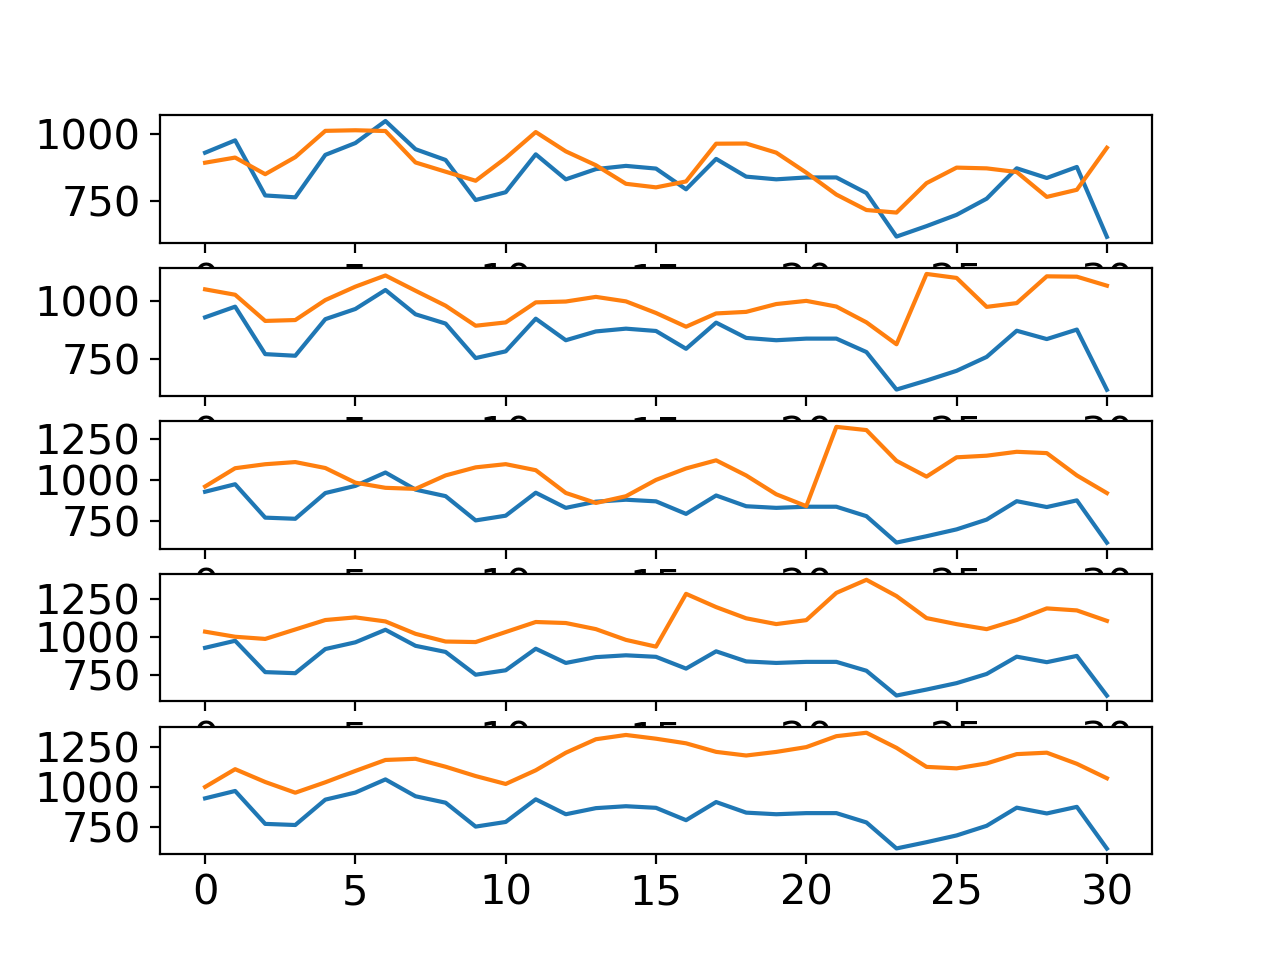
\includegraphics[width=\textwidth]{./results/images/realvspredicted}

     \caption{NRMSE for different prediction window ranges}\label{fig:realvspredicted}
 \end{figure}
 